\documentclass[letterpaper,11pt]{article}
\oddsidemargin -1.0cm \textwidth 17.5cm

\usepackage[utf8]{inputenc}
\usepackage[activeacute,spanish, es-lcroman]{babel}
\decimalpoint
\usepackage{amsfonts,setspace}
\usepackage{amsmath}
\usepackage{amssymb, amsmath, amsthm}
\usepackage{comment}
\usepackage{float}
\usepackage{amssymb}
\usepackage{dsfont}
\usepackage{anysize}
\usepackage{multicol}
\usepackage{enumerate}
\usepackage{graphicx}
\usepackage[left=1.5cm,top=2cm,right=1.5cm, bottom=1.7cm]{geometry}
\setlength\headheight{1.5em} 
\usepackage{fancyhdr}
\usepackage{multicol}
\usepackage{hyperref}
\usepackage{wrapfig}
\usepackage{subcaption}
\usepackage{siunitx}
\usepackage{cancel}
\usepackage{mdwlist}
\usepackage{svg}
\pagestyle{fancy}
\fancyhf{}
\renewcommand{\labelenumi}{\normalsize\bfseries P\arabic{enumi}.}
\renewcommand{\labelenumii}{\normalsize\bfseries (\alph{enumii})}
\renewcommand{\labelenumiii}{\normalsize\bfseries \roman{enumiii})}


\begin{document}

\fancyhead[L]{\itshape{Facultad de Ciencias F\'isicas y Matem\'aticas}}
\fancyhead[R]{\itshape{Universidad de Chile}}

\begin{minipage}{11.5cm}
    \begin{flushleft}
        \hspace*{-0.6cm}\textbf{FI1000-1 Introducción a la Física Clásica}\\
        \hspace*{-0.6cm}\textbf{Profesora:} Jocelyn Dunstan\\
        \hspace*{-0.6cm}\textbf{Auxiliar:} Alejandro Silva\\
        \hspace*{-0.6cm}\textbf{Ayudantes:} Macarena Muñoz \& Catalina Vargas\\
    \end{flushleft}
\end{minipage}

\begin{picture}(2,3)
    \svgpath{../}  % descomentar si se agrega a carpeta "auxiliares"/"ejercicios"
    \put(366, 10){\includesvg[scale=0.31]{img/dfi.svg}}
\end{picture}

\begin{center}
	\LARGE\textbf{Ejercicio \#8}\\
	\Large{Choques inelásticos}
\end{center}

\vspace{-1cm}
\begin{enumerate}\setlength{\itemsep}{0.4cm}

\rfoot[]{pág. \thepage}

\item[]

\item A y B son dos esferitas de igual masa m engarzadas en el eje horizontal. B
está unida a un resorte ideal de largo natural $l_0$ y rigidez $k$. Inicialmente B está en reposo, el resorte en dirección vertical y sin deformación. A se desliza con velocidad $v$ \textbf{desconocida}, choca con B y ambas permanecen unidas tras la colisión. Calcular $v$, si en el instante en que el
conjunto se detiene el ángulo $\theta$ tiene un valor de $60^o$. Suponga que el roce es
despreciable.

\begin{figure}[H]
    \centering
    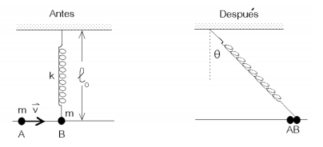
\includegraphics[width=10cm]{2021-2/img/ejercicios/ej8.PNG}
    \caption{Caption}
    \label{fig:ej8}
\end{figure}
Formulario:

\begin{equation}
    P_{final}=P_{inicial}
\end{equation}

\begin{equation}
    E_{resorte}=\frac{1}{2}k(\Delta x)^2
\end{equation}

\begin{equation}
    E_{cinetica}=\frac{1}{2}mv^2
\end{equation}

\begin{equation}
    a^2+b^2=c^2
\end{equation}

\begin{equation}
    cos(60^o)=\frac{1}{2}
\end{equation}
% Para imágenes vectoriales -> el texto tiene que estar en LaTeX
% \begin{figure}[htbp]
%   \centering
%   \svgpath{../Imagenes/ejercicios}  -> .. irse pa'trás 
%   \includesvg{ej5.svg}
% \end{figure}

\end{enumerate}
\end{document}